\documentclass[addpoints]{exam}
\usepackage{amsmath,amsthm,amssymb,url}

\usepackage{algorithm}
\usepackage{algorithmic}
\usepackage{graphicx}
\usepackage{float}
\usepackage[pdftex]{hyperref}
\usepackage{tikz}


\newtheorem{lemma}{Lemma}[section]
\newcommand{\var}{\text{Var}}
\title{CS 6150: Homework 4}
\date{Due Date: November 20, 2015}
\author{Christopher Mertin}
\begin{document}
\maketitle
\begin{center}
\fbox{\fbox{\parbox{5.5in}{\centering
This assignment has \numquestions\ questions, for a total of \numpoints\
points.
Unless otherwise specified, complete and reasoned arguments will be
expected for all answers. 
}}}
\end{center}

\qformat{Question \thequestion: \thequestiontitle\dotfill \textbf{[\totalpoints]}}
\pointname{}
\bonuspointname{}
\pointformat{[\bfseries\thepoints]}

\printanswers

\begin{center}
  \gradetable
\end{center}
\newpage



\begin{questions}


\titledquestion{Cycle Cover}[20]
A cycle cover $C$ of a directed graph $G(V,E)$ is a collection of
vertex-disjoint directed cycles so that each vertex in V belongs to
some cycle in $C$.

Give a polynomial time algorithm to compute a cycle cover of a given
directed graph, or correctly report that one does not exist.

\begin{solution}
There exists a cycle cover if there exists a perfect matching for the graph. If a perfect matching does not exist, then there is no disjoint cycle cover. Therefore, finding the cycle cover can be reduced into the perfect matching problem.

From the original graph $G$, we can create a bipartite graph $G^{\prime}$. To do this, take the original set of vertices and have them be in their own set $\mathcal{L}=\{u_{1},u_{2},\ldots,u_{n}\}$ to be the left side of the bipartite graph, and create a {\em copy} of each vertex and have it be in the set $\mathcal{R}=\{u_{1}^{\prime},u_{2}^{\prime},\ldots,u_{n}^{\prime}\}$ to be the right side of the bipartite graph. There is a source vertex $s$ that has an edge $\left(s, u_{\mu}\right)\ \forall\ \mu=\{1,2,\ldots,n\}$ and a target vertex $t$ that has an edge $\left(u_{\gamma}^{\prime},t\right)\ \forall\ \gamma=\{1,2,\ldots,n\}$. This would take $\mathcal{O}(2VE)$ to build.

From here, we can draw an edge from $\mathcal{L}$ to $\mathcal{R}$ reprsenting each edge that existed in the original graph. For example, if the edge $\left(u_{1},u_{5}\right)$ was in the original graph $G$, then the edge $\left(u_{1},u_{5}^{\prime}\right)$ is in the graph $G^{\prime}$. This will create a bipartite graph that holds the same information as was in $G$.

{\bf EdmondsKarp}$(G)${\bf:}
\vspace{-1em}\begin{enumerate}
\itemsep-0.5em
\item $f\leftarrow 0;\quad G_{f}\leftarrow G$
\item {\bf while} $G_{f}$ contains an $s$-$t$ path $P$ {\bf do}

\item\hspace{3em}Let $P$ be an $s$-$t$ path in $G_{f}$ with the minimum number of edges

\item\hspace{3em}Augment $f$ using $P$

\item\hspace{3em}Update $G_{f}$

\item {\bf end while}
\item {\bf return} $f$
\end{enumerate}
\vspace{-1em}
Finally, we can use a Bipartite Matching Algorithm to get the mathching from $G^{\prime}$. This will return the set of vertices that are connected in the directed graph which, if it is a perfect matching, will represent the vertex-disjoint directed cycle cover of $G$. A polynomial algorithm such as the Edmonds-Karp Algorithm can be used to solve this in $\mathcal{O}\left(VE^{2}\right)$, which was proven in class, resulting in an overall computation time of $\mathcal{O}\left( VE^{2} + 2VE\right)$.
\end{solution}


\titledquestion{Attend all lectures}[20]
There are $n$ lectures with start time $s_{i}$, end time $e_{i}$
and $t_{ij}$ being the time spent in going from lecture $i$ to $j$.
Now a group of students wants to attend all of the lectures by
sending no more than one student to each lecture. Assume $s_{i}, e_{i},
t_{ij}$ are all positive integers.

Find an algorithm that minimizes number of students covering all the
lectures.

\begin{solution}
The question asks if there is a way to minimize the number of students that attend classes, so if a student is able to attend class $i$ and then immediately leave for class $j$, then a new student doesn't have to be ``dispatched." Therefore, a bipartite graph $G$ can be created such that a {\em maximum matching} can be used to divide up the courses.%such that each set represents students who attend more than one lecture, and students who just attend a few when none of the other set can make it.

For each of the classes $i = \left\{ 1,2,\ldots,n\right\}$, there are two nodes $\mathcal{L}=\left\{ \ell_{1}, \ell_{2}, \ldots, \ell_{n}\right\}$ and $\mathcal{R}=\left\{ r_{1}, r_{2}, \ldots, r_{n} \right\}$, where $\mathcal{L}$ is the left group of the bipartite graph which represents all the courses, and $\mathcal{R}$ the right which represents all courses that a student can attend right after attending another one. For each lecture $i$ and $j$, for $i < j$, if $s_{j}\geq e_{i} + t_{ij}$, then we can draw a directed edge from $\left( \ell_{i},r_{j} \right)$.


{\bf Bipartite Matching}$(G,M)${\bf:}
\vspace{-1em}\begin{enumerate}
\itemsep-0.5em
\item Start a Depth First Search at a vertex in $\mathcal{L}$
\item if current vertex $\leftarrow \mathcal{L}$

\item \hspace{2.5em} follow an edge $e\in M$

\item else

\item\hspace{2.5em} follow an edge $e\notin M$

{\em If at any point we find an unmatched vertex in $\mathcal{R}$, then the augmenting path is found.}
\end{enumerate}
\vspace{-.75em}
We can define a variable $M$ as the maximum matching of the bipartite graph, which the alogrithm is defined above. This minimum number of students who can attend the lecture can be defined as $n - \left| M \right|$, as $\left| M\right|$ would represent the number of students who attend one or more lectures. This is the optimal solution for minimizing the number of students who are attending the lecture.

This statement can be proven via {\em proof by contradiction}. Assume that this can be done with less students, $\xi$, such that $n-\xi < n - \left| M \right|$. We can define two {\em alternative sets} $\mathcal{I} = \left\{ i_{1}, i_{2}, \ldots, i_{\xi} \right\}$, which represents the set of lectures where students attend more than one, and $\mathcal{J} = \left\{ j_{1}, j_{2}, \ldots, j_{\xi}\right\}$ which represents all of the classes that were attended after lectures in $\mathcal{I}$. From here, we can create a matching, $M^{\prime} = \left\{ \left(\ell_{i_{1}}, r_{j_{1}} \right), \left(\ell_{i_{2}}, r_{j_{2}} \right), \ldots, \left(\ell_{i_{\xi}}, r_{j_{\xi}} \right)  \right\}$, which would minimize the set as it's a matching in the graph. Note that $\xi = \left| M^{\prime}\right|$. Since $M^{\prime}$ is a matching in $G$, this implies that $\left| M^{\prime}\right| = \left| M\right|$ as they should be the same values since all lectures need to be attended. However, the original assumption was that $\xi > \left| M\right|$, which was a contradiction. Therefore, $n-\left| M\right|$ is the minimum limit on the number of students to attend all the lectures.

\end{solution}


\titledquestion{Monotone path}

Solve all parts of question 2 in
\url{http://web.engr.illinois.edu/~jeffe/teaching/algorithms/notes/25-maxflowext.pdf}

Breakdown is $5$ + $5$ + $10$.

Suppose we are given an $n\times n$ grid, some of whose cells are marked; the grid is represented by an array $M[1\ldots n, 1\ldots, n]$ of booleans, where $M[i,j]=\text{{\sc True}}$ if and only if cell $(i,j)$ is marked. A {\em monotone} path through the grid starts at the top-left cell, moves only right or down at each step, and ends at the bottom-right cell. Our goal is to cover the marked cells with as few monotone paths as possible.

\begin{figure}[!h]
\centering
\includegraphics[width = .9\textwidth]{4_img.png}
\caption{Greedily covering the marked cells in a grid with four monotone paths.}
\end{figure}

\begin{parts}
\part[5] Describe an algorithm to find a monotone path that covers the largest number of marked cells.

\begin{solution}
As the question didn't mention efficiency, this can be done via a brute-force method. First construct the graph such that each cell is an individual node from $\left\{ u_{1,1},u_{1,2},\ldots,u_{n,n}\right\}$. Draw directed edges, if they exist, for all nodes from $\left( u_{i,j},u_{i+1,j} \right)$ and $\left( u_{i,j},u_{i,j+1} \right)$ to restrict movements in the graph to those defined in the problem. Finally, if a node represents a cell that is marked, give it a value of $1$, else the node has a value of $0$.

To find the path that coveres the {\em largest} number of marked cells, an algorithm such as {\em Depth First Search} or {\em Breadth First Search} can be used to determine all of the paths that are in the graph. The values of nodes traversed can be recorded such that after figuring out all of the paths, the path which traversed the largest number of marked cells would have the largest value. This solution does not need a proof as it is looking at all possible paths and choosing the largest of the set, and is trivially true.
\end{solution}

\part[5] There is a natural greedy heuristic to find a small cover by monotone paths: If there are any marked cells, find a monotone path $\pi$ that covers the largest number of marked cells, unmark any cells covered by $\pi$ those marked cells, and recurse. Show that this algorithm does {\em not} always compute an optimal solution.

\begin{solution}
This can be shown via proof by contradiction. We can assume that if there are multiple paths with the same {\em largest} number of marked cells in it, then one will be chosen at random. This image can be seen below.

\begin{center}
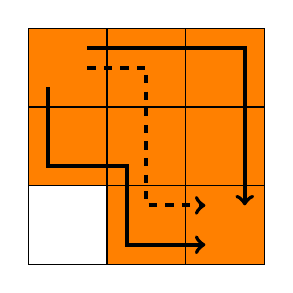
\begin{tikzpicture}
\draw[] (0,0) rectangle (1,1);
\draw[fill=orange] (0,1) rectangle (1,2);
\draw[fill=orange] (0,2) rectangle (1,3);

\draw[fill=orange] (1,0) rectangle (2,1);
\draw[fill=orange] (1,1) rectangle (2,2);
\draw[fill=orange] (1,2) rectangle (2,3);

\draw[fill=orange] (2,0) rectangle (3,1);
\draw[fill=orange] (2,1) rectangle (3,2);
\draw[fill=orange] (2,2) rectangle (3,3);

\draw[->, line width=.5mm] (.25,2.25) -- (.25,1.25) -- (1.25,1.25) -- (1.25,.25) -- (2.25,.25);
\draw[->, line width=.5mm, dashed] (.75,2.5) -- (1.5,2.5) -- (1.5,1.5) -- (1.5,.75) -- (2.25,.75);
\draw[->, line width=.5mm] (.75,2.75) -- (2.75,2.75) -- (2.75, .75);
\end{tikzpicture}
\end{center}
Each of the paths in the above figure represent possible paths with the {\em largest} number of marked cells. The optimal {\em first path} to be chosen would be either solid line, as if either is chosen then all of the marked nodes can be visited with only 2 monotone paths. However, the dashed line would take a total of 3 monotone paths to visit all of the marked nodes if it is chosen first. Therefore, simply going by the number of marked nodes visited is not sufficient to produce the minimum number of monotone paths with each iteration. 
\end{solution}



\part[10] Describe and analyze an efficient algorithm to compute the smallest set of monotone paths that covers every marked cell.
\begin{solution}
This can be done by constructing a directed graph $G$ as follows:

\begin{enumerate}
\item For each index in the array $M[i,j]$, create two vertices $u_{i,j}$ and $v_{i,j}$, the source vertex $s$ and the target vertex $t$. This will create $\mathcal{O}\left( 2n^{2}+2\right)$ vertices.
\item Each $u_{i,j}$ has a directed egde $\left( u_{i,j},v_{i,j} \right)$, where the edge will have a demand $1$ if $M[i,j]$ is {\sc True} and $0$ if it is {\sc False}. Each of these edges have no capacity, as each monotone path is independent of the other as they can overlap in cells. This creates $\mathcal{O}\left( n^{2} \right)$ edges.
\item Give each vertex in $v_{i,j}$ a directed edge from $\left( v_{i,j},u_{i+1,j} \right)$ and $\left( v_{i,j},u_{i,j+1} \right)$ with no demand and no capacity, for the same reasons stated above. This creates $\mathcal{O}\left( 2n^{2}\right)$ edges as well, resulting in $\mathcal{O}\left( 3n^{2}\right)$ total edges.
\item Create an edge $\left( s, u_{1,1}\right)$ from the source to the first cell with no demand and no restrictions on capacity. We choose to not restrict the capacity of this vertex as we don't know what the capacity of the mincut is going to be yet. We do the same for the target, by creating the edge $\left(v_{n,n},t \right)$ with again no demand and no restrictions on capacity. We can use a max flow algorithm on this new graph. 
\end{enumerate}

%For each index in the array $M$, there exists two vertices $u_{i,j}$ and $v_{i,j}$, and the source vertex $s$. We can build $G$ such that each $u_{i,j}$ has a directed egde $\left( u_{i,j},v_{i,j} \right)$, where the edge will have a demand $1$ if $M[i,j]$ is {\sc True} and $0$ if it is {\sc False}.

%Finally, we can give each vertex in $v_{i,j}$ a directed edge from $\left( v_{i,j},u_{i+1,j} \right)$ and $\left( v_{i,j},u_{i,j+1} \right)$ with no demand and no capacity, and an edge from $\left( s,u_{1,1} \right)$ with a capacity of $k$.

This above method creates $\mathcal{O}\left( n^{2}\right)$ vertices and $\mathcal{O}\left( n^{2}\right)$ edges and restrict the movement to those contraints in the question. From here, a max flow algorithm such as Orlin's Max Flow Algorithm can be used to calculate the maximum flow in $\mathcal{O}(VE)$ time, which is $\mathcal{O}\left( n^{4}\right)$ which will produce the minimum number of edges that would coincide with all the marked cells. This would produce the $k$-monotone paths since the max flow algoirthms minimize the number of paths required to receive the maximum flow, {\em i.e.} contain all of the marked cells.

%This will create a network of paths that would represent a structure similar to the original grid with $\mathcal{O}\left( n^{2}\right)$ vertices and edges, while also restricting the movement to those moves defined in the problem. All of the directed edges will represent a path in which to reach the final node $v_{n,n}$. An efficient mmax flow algorithm can be comptued on this graph in $\mathcal{O}\left( n^{4}\log(n)\right)$ time to produce the $k$-monotone edges that would coincide with all the marked cells.
\end{solution}
\end{parts}

\titledquestion{Vertex-disjoint paths}[20]
Given a square grid $(n\times n)$ like the following figure, and a set of $m
\leq n^{2}$ distinct points marked in black, devise an algorithm to
determine whether there exists $m$ vertex-disjoint paths starting at
those marked points and ending at points at the boundary of the grid.

\begin{figure}[H]
  \centering
  \includegraphics[width=0.75\textwidth]{grid.png}\\
  \caption{In the left grid there exists such a path, but in the right
  grid there isn't}
\end{figure}

\begin{solution}

%%%%%%%%%%%%%%%%%%%%%%%%%% Known as the escape problem

The solution to this can be a {\em Multi-source multi-sink maximum flow problem} \cite{wiki-Multi} problem by building a graph $G$ to the following specifications:

\begin{enumerate}
\item Create a vertex for each node in the graph, resulting in $n^{2}$ vertices.
\item For each of the $m$ starting points, treat them as a ``source point'' by labeling them as $s_{\mu}$, where superceeding these is an ``official'' source $s$ that has a directed edge $\left( s, s_{\mu}\right)\ \forall\ \mu=\{1,2,\ldots,m\}$.
\item Assign each of the $4n - 4$ boundary nodes as a target vertex, $t_{\gamma}$, with an ``official'' target $t$ that has a directed edge $\left( t_{\gamma}, t\right)\ \forall\ \gamma=\{1,2,\ldots,4n-4\}$.
\item Build the connections as from the images above. For example, the first node, $u_{1,1}$ has neighbors $u_{2,1}$ and $u_{1,2}$ so an edge needs to be drawn to both. However, instead of having an undirected edge, make it two directional edges, one for each direction. In other words, create edges $\left(u_{1,1},u_{1,2}\right)$ and $\left( u_{1,2}, u_{1,1}\right)$ for each of the edges so that {\em either} direction is possible on the grid.
\item Finally, give all edges and vertices in the graph a capacity of $1$.
\end{enumerate}

Step $4$ allows for flow in any of the directions, while step $5$ restricts any overlap. Finally, we can use a max flow algorithm such as Edmonds-Karp to tell the number of vertex-disjoint paths in $G$. We can define the calculated maximum flow as $\vartheta$, such that the value of $\vartheta$ represents the number of vertex-disjoint paths. Therefore if $\vartheta = m$, then $m$ vertex-disjoint paths exist.

Dr. Venkatasubramanian stated that my work needed to prove that the max flow of a graph is the same as the number of vertex-disjoint paths, so this is what this does via {\em proof by contradiction}. First, we assume that if the max flow of $G$ is $\vartheta$, then there should be some other parameter $\xi$ which represents the number of vertex-disjoint paths, such that $\xi \neq \vartheta$. If this is true, then there should never be any instance which $\xi = \vartheta$. 

Suppose that there are $m$ ``source points,'' with $\lambda$ of those nodes being on the boundary, in other words at $t_{\gamma}$, and $\lambda \leq m$. If $\lambda$ is large enough to cover all the boundary vertices, then one of two scenarios occurs:

\begin{enumerate}
\itemsep-0.5em
\item {\bf If $\lambda < m$:} The figure below represents the type of graph that is being discussed here, with the red points representing the source points and the black points representing those which aren't sources. Recall that the above statement assumes that there are $\lambda$-vertices along the boundary of the grid. Therefore there are $(m - \lambda)$ source vertices that are {\em inside} the grid. However, looking at the given algorithm to build the graph, each of the vertices is given a capacity of one in step 5, so no vertices inside the grid can utilize any of the targets $t_{\gamma}$ for $\gamma=\{1,2,\ldots,\lambda\}$. The maximum flow and number of vertex-disjoint paths of the graph is $\xi = \vartheta = \lambda < m$. 

\begin{center}
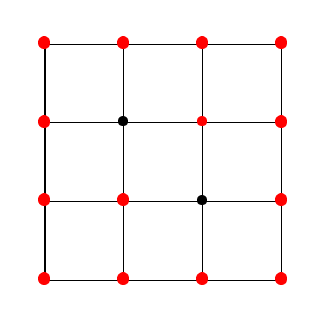
\begin{tikzpicture}
\draw (0,0) -- (0,3);
\draw (3,0) -- (0,0);
\draw (1,0) -- (1,3);
\draw (3,1) -- (0,1);
\draw (2,0) -- (2,3);
\draw (3,2) -- (0,2);
\draw (3,0) -- (3,3);
\draw (3,3) -- (0,3);

\node[red] at (0,0) {{\large \textbullet}};
\node[red] at (0,1) {{\large \textbullet}};
\node[red] at (0,2) {{\large \textbullet}};
\node[red] at (0,3) {\large \textbullet};

\node[red] at (1,0) {{\large \textbullet}};
\node[red] at (1,1) {\large \textbullet};
\node at (1,2) {\textbullet};
\node[red] at (1,3) {\large \textbullet};

\node[red] at (2,0) {\large \textbullet};
\node at (2,1) {\textbullet};
\node[red] at (2,2) {\textbullet};
\node[red] at (2,3) {\large \textbullet};

\node[red] at (3,0) {\large \textbullet};
\node[red] at (3,1) {\large \textbullet};
\node[red] at (3,2) {\large \textbullet};
\node[red] at (3,3) {\large \textbullet};
\end{tikzpicture}
\end{center}

\item {\bf If $\lambda = m$:} The figure below shows the type of graph that is being discussed, with the red points representing the source points.  Then it can trivially be seen that the max flow is $\lambda$, as $\lambda$ ``source points'' flow directly to all the target vertices. In other words, $\xi = \vartheta = \lambda = m$. 

\begin{center}
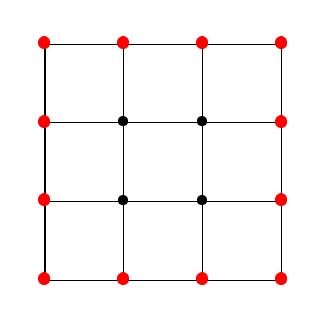
\begin{tikzpicture}
\draw (0,0) -- (0,3);
\draw (3,0) -- (0,0);
\draw (1,0) -- (1,3);
\draw (3,1) -- (0,1);
\draw (2,0) -- (2,3);
\draw (3,2) -- (0,2);
\draw (3,0) -- (3,3);
\draw (3,3) -- (0,3);

\node[red] at (0,0) {{\large \textbullet}};
\node[red] at (0,1) {{\large \textbullet}};
\node[red] at (0,2) {{\large \textbullet}};
\node[red] at (0,3) {\large \textbullet};

\node[red] at (1,0) {{\large \textbullet}};
\node at (1,1) {\textbullet};
\node at (1,2) {\textbullet};
\node[red] at (1,3) {\large \textbullet};

\node[red] at (2,0) {\large \textbullet};
\node at (2,1) {\textbullet};
\node at (2,2) {\textbullet};
\node[red] at (2,3) {\large \textbullet};

\node[red] at (3,0) {\large \textbullet};
\node[red] at (3,1) {\large \textbullet};
\node[red] at (3,2) {\large \textbullet};
\node[red] at (3,3) {\large \textbullet};
\end{tikzpicture}
\end{center}
\end{enumerate}

Therefore, it was shown in the extreme case that $\xi = \vartheta$ on all orientations of the graph. However, the original assumption stated that $\xi \neq \vartheta$, which is a contradiction. Thus, the value of the {\em maximum flow} is the number of vertex-disjoint paths in the set.

Finally, due to the constraints imposed by the algorithm, such as in step 4 to allow for movement in any direction and in step 5 to restrict overlapping edges and vertices, the max flow would be equal to the capacity of the number of sources that made it to the boundary. This is because the flow of each source point would be 1 and the resulting flow at $t$ would be the number of sources that made it to the target. In other words, if $\vartheta = m$ then there are $m$ vertex-disjoint paths.

\end{solution}

\titledquestion{Uniqueness of mincut}[20]
Given an $s$-$t$ flow network, find a polynomial time algorithm to
determine whether the mincut is unique.

\begin{solution}
This is assuming that the mincut has already been computed with an algorithm in polynomial time. 

This computed mincut contains $k$-edges, where the cutting of these edges would interrupt the flow from $s$ to $t$. These edges from the cut belong to the set $\mathcal{E}=\{e_{1},e_{2},\ldots,e_{k}\}$, which belong to the mincut $C$. The {\em value} of this mincut is represented by $\left| C\right|$, which represents the sum of all the values of the edges in $\mathcal{E}$.

For each of the edges in $\mathcal{E}\in C$, we can individually increase the capacity of each edge {\em one at a time}. As we iterate through the edges, each time we increase the capacity of an edge in $\mathcal{E}$, we calculate a new mincut, $C_{i}$, after which we set the capacity of that edge back to the original value before moving on to the next edge. 

From this, we can conclude if the mincut is unique. If $\left| C \right| = \left| C_{i}\right|$ for any $i$, then we can say that the original mincut is {\em not unique}. This is due to the fact that we increased our capacity on an edge by 1, so if it was unique for that value then we shouldn't get the same value of $\left| C\right|$. On the other hand, if $\left| C \right| = \left| C_{i}\right| - 1$ for all $i = \{1, 2, \ldots, k\}$, then we can say that the mincut is {\em unique}.

This would produce a polynomial time algorithm depending on the algorithm used to calculate the mincut. For example, using the Edmonds-Karp algorithm caluclates a single mincut in $\mathcal{O}\left( VE^{2}\right)$, so using it in conjunction with the above algorithm to calculate the ``new mincuts'' produces a $\mathcal{O}\left( k\cdot VE^{2}\right)$ algorithm to check to see if a given mincut is unique.
\end{solution}

\end{questions}

\begin{thebibliography}{99}
\bibitem{wiki-Multi}\url{https://en.wikipedia.org/wiki/Maximum_flow_problem#Multi-source_multi-sink_maximum_flow_problem}
\end{thebibliography}

\end{document}

%%% Local Variables:
%%% mode: latex
%%% TeX-master: t
%%% End:
